% Build from this directory (TeX Live with TikZ and dvisvgm):
% latex -interaction=nonstopmode -halt-on-error pam-6.tex
% dvisvgm --no-fonts --exact --bbox=papersize pam-6.dvi -o pam-6.svg
\documentclass[tikz,border=4pt]{standalone}
\usetikzlibrary{arrows.meta}
\definecolor{positionblue}{HTML}{4472C4}
\definecolor{positionorange}{HTML}{ED7D31}
\definecolor{positionborder}{HTML}{305496}
\begin{document}
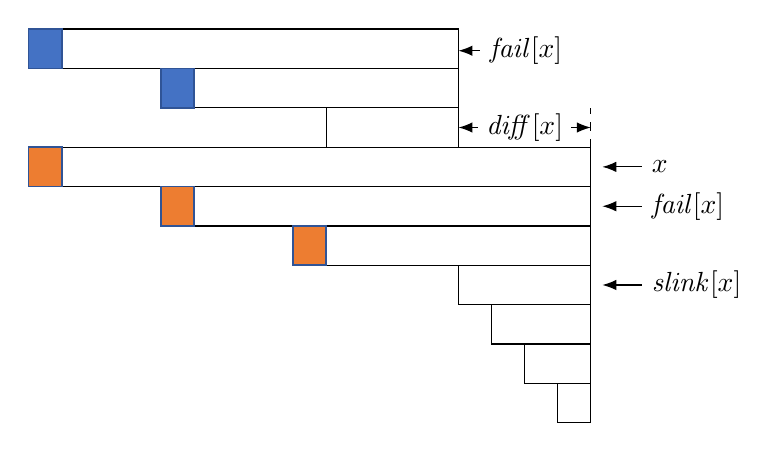
\begin{tikzpicture}[x=0.42cm,y=0.5cm,line width=0.45pt,
  >=Latex,font=\normalsize]
  % The earlier occurrence ends at i-diff[x]. Its two blue positions
  % contribute g[fail[x]] and align with the first two orange positions.
  \draw (0,9) rectangle (13,10);
  \draw (4,8) rectangle (13,9);
  \draw (9,7) rectangle (13,8);
  \foreach \left/\bottom in {0/9,4/8} {
    \filldraw[fill=positionblue,draw=positionborder,line width=0.65pt]
      (\left,\bottom) rectangle ++(1,1);
  }

  % Palindromic suffixes ending at i. The first three form the series
  % contributing to g[x]; slink[x] belongs to the following series.
  \foreach \left/\bottom in {0/6,4/5,8/4,13/3,14/2,15/1,16/0} {
    \draw (\left,\bottom) rectangle (17,\bottom+1);
  }
  \foreach \left/\bottom in {0/6,4/5,8/4} {
    \filldraw[fill=positionorange,draw=positionborder,line width=0.65pt]
      (\left,\bottom) rectangle ++(1,1);
  }

  % The difference in the two ending positions is exactly diff[x].
  \draw[dashed] (17,7) -- (17,8);
  \draw[<->] (13,7.5) -- (17,7.5)
    node[midway,fill=white,inner xsep=3pt,inner ysep=0.5pt]
      {$\mathit{diff}[x]$};

  \draw[<-] (13,9.45) -- (13.65,9.45)
    node[right] {$\mathit{fail}[x]$};
  \draw[<-] (17.35,6.5) -- (18.55,6.5) node[right] {$x$};
  \draw[<-] (17.35,5.5) -- (18.55,5.5)
    node[right] {$\mathit{fail}[x]$};
  \draw[<-] (17.35,3.5) -- (18.55,3.5)
    node[right] {$\mathit{slink}[x]$};
\end{tikzpicture}
\end{document}
